\section{Introduction}
The versatility of snickerdoodle is due to it's software definable and reconfigurable hardware interface. The on-board Zynq-7000's programmable logic allows for the hardware interface to be defined by a bitstream that can be generated in a way that is exceedingly similar to software and application development. The development environment, Vivado\textregistered, has been architected in such a way that the transition between developing for the programmable logic (PL) and processing subsystems (PS) is seamless. \\


\margininfonote{Portions of this guide have been excerpted and adapted from the Xilinx\textregistered\ Wiki found at \url{http://www.wiki.xilinx.com/}}

\noindent
This guide will get you started developing hardware definitions for snickerdoodle. In this guide, it is assumed that you have an installation of Vivado (this guide uses the 2015.4 release) on a host computer. The process outlined in this guide was created using Ubuntu 14.04 as the host computer operating system. While the process is similar for Windows users, those using Windows operating systems should consult the Windows version of this guide. \\



\begin{figure*}
	\centering
	
\includegraphics{images/Hardware_Process.pdf}
	\caption{Hardware Configuration Process}
	\label{fig:hardwareconfigprocess}
\end{figure*}



\section{Install snickerdoodle Board Files}
To begin working with programmable logic on snickerdoodle, a set of board files need to be installed onto the host computer for access by Vivado. The board files are a set of text files that are read by Vivado on startup and provide a set of constraints that define the board hardware. \\

\subsection{Download Board Files}
The board files can be downloaded directly from \href{https://github.com/krtkl/snickerdoodle-board-files}{GitHub}. The files can be downloaded as a \texttt{.zip} file from a web browser, downloaded directly using \texttt{wget} or cloned using \texttt{git clone}. \\



\noindent
The archive (\texttt{.zip}) can be downloaded directly from the command line by invoking \texttt{wget}. The following command will download the board files repository archive:

\begin{fullwidth}
\begin{lstlisting}[style=text]
wget https://github.com/krtkl/snickerdoodle-board-files/archive/master.zip
\end{lstlisting}
\end{fullwidth}


\subsection{Installing Board Files}

\margincautionnote{Moving or copying files into the Vivado install directory will require root permissions just as installing any program would.}

After downloading the board files archive, the files will need to be installed in the proper location so that they may be read by Vivado. The directory that Vivado uses to load board files when starting is relative to it's install location. Typically, Vivado is installed at \texttt{/opt/Xilinx/Vivado/<release>}. The board files are located at \texttt{<vivado\_install\_dir>/data/boards/board\_files}. In this example, the board files will be copied to the corresponding directory of a 2015.4 release. \\

\noindent
The only files that should be installed are the \texttt{snickerdoodle} and \texttt{snickerdoodle\_black} directories which contain the board files for the corresponding snickerdoodle version. An exclusion file (\texttt{EXCLUDE}) is included in the archive to help with the copying process and prevent extraneous files (documentation, README, etc.) from being copied into the board files directory. \\

\noindent
The following series of commands will extract the \texttt{.zip} archive and move the resulting board files into the \texttt{board\_files} directory: \\

\begin{fullwidth}
\begin{lstlisting}[style=text]
$ wget https://github.com/krtkl/snickerdoodle-board-files/archive/master.zip
$ unzip master.zip
$ cd snickerdoodle-board-files-master
$ rsync -av --exclude-from=EXCLUDE ./* /opt/Xilinx/Vivado/2015.4/data/boards/board_files/
\end{lstlisting}
\end{fullwidth}

\noindent
Once the board files have been installed, Vivado will need to be restarted to load the files from the data directory.

\section{Creating a New Project}

Creating a new project can be done by selecting \texttt{\bfseries File $\rightarrow$ New Project...} from the menubar or by selecting the \textit{Create New Project} icon from the "Quick Start" menu, as shown in \figref{fig:vivadostartcreate}. \\


\begin{figure}
	\centering
	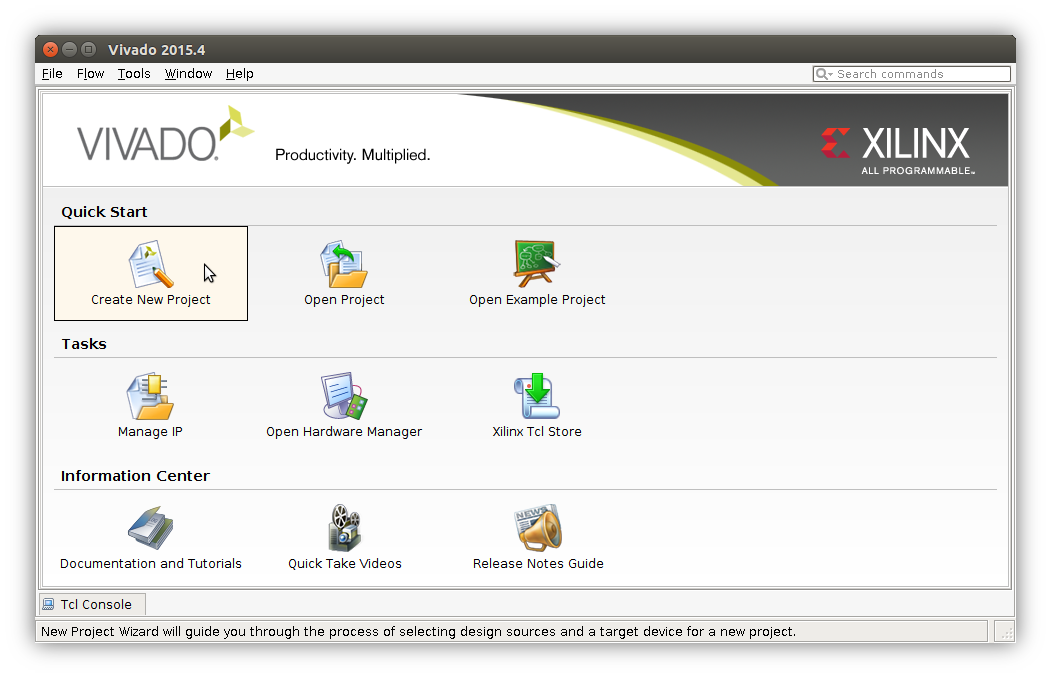
\includegraphics{images/Vivado_Start_Create_Project.png}
	\caption[Vivado Startup Create New Project]{Vivado Startup Create New Project}
	\label{fig:vivadostartcreate}
\end{figure}


\noindent
The first step to creating a new Vivado project is to select the project name and parent directory. By default, Vivado will create a new subdirectory for which to store the project files. It is highly recommended that this setting be left unchanged to keep the project files and directories organized and easily accessible for development (\ie from the SDK). \figref{fig:vivadonewprojectname} shows the input of the project name and parent directory when creating a new project. \\

\begin{figure}
	\centering
	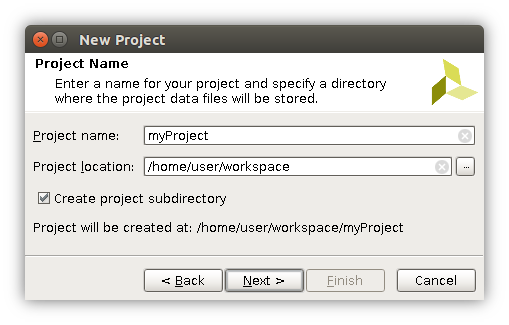
\includegraphics{images/New_Project}
	\caption{Selecting Project Name and Parent Directory}
	\label{fig:vivadonewprojectname}
\end{figure}

\subsection{Project Type and Sources}
At this point in the project creation process, IP and design sources can be added to the project. If you would like to include existing sources, you will prompted to include those before choosing a project board. If you choose not to include any existing assets or constraints, the "Do no specify sources..." checkbox, shown in \figref{fig:newprojecttype}, can be selected to skip this step. Sources can be added to the project at any time after creation as outlined \hyperref[sub:addsources]{below}.\\

\begin{figure}
	\centering
	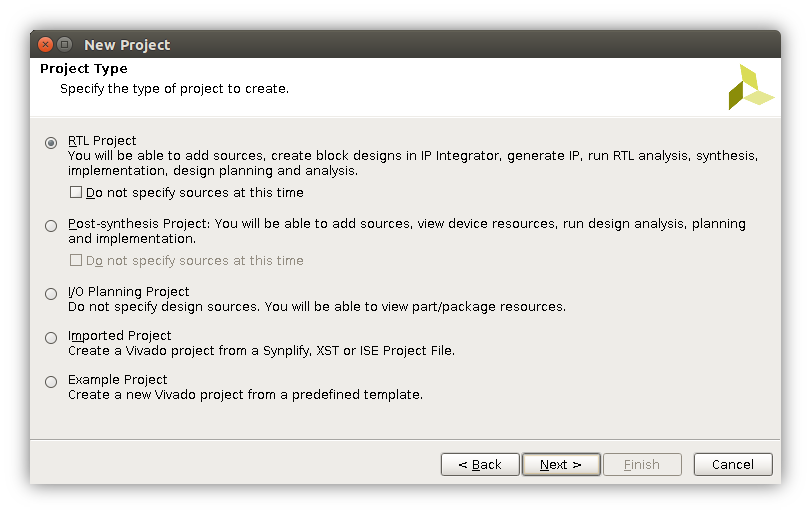
\includegraphics{images/New_Project_Type.png}
	\caption{Project Type Selection Dialog}
	\label{fig:newprojecttype}
\end{figure}


\newpage

\subsection{Choosing a Project Board}
If the board files have been copied and loaded properly, they will be listed in the table of boards. To view the available boards, choose "Boards" rather than "Parts" at the top of the window as shown in \figref{fig:vivadoprojectboard}. \\

\begin{figure}
	\centering
	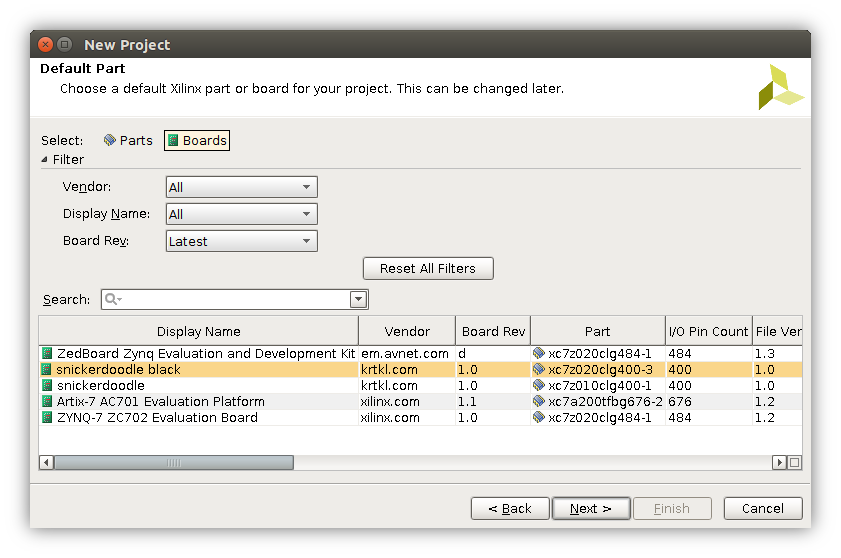
\includegraphics{images/Project_Boards.png}
	\caption{Selecting a Project Board}
	\label{fig:vivadoprojectboard}
\end{figure}

\noindent
After selecting a board, the details of the project will be listed in the \textit{New Project Summary} shown in \figref{fig:vivadoprojectfinish}. By clicking the "Finish" button, the project will be created and opened in the Vivado graphical user interface (GUI). \\

\begin{figure}
	\centering
	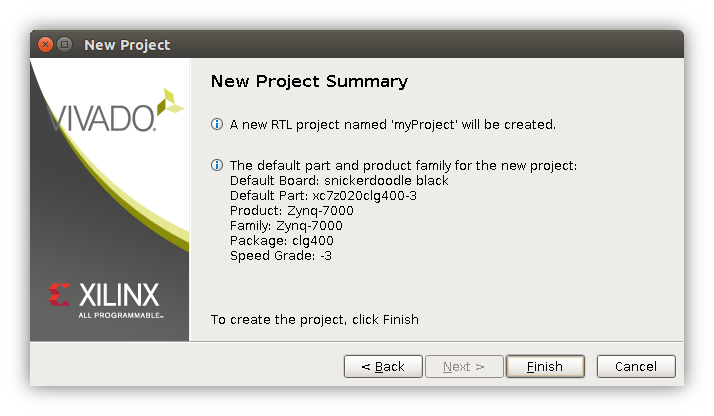
\includegraphics{images/Finish_New_Project.png}
	\caption{Review and Finish New Project Creation}
	\label{fig:vivadoprojectfinish}
\end{figure}


\section{Working with Vivado}
%\margininfonote{Additional information and resources on using Vivado to create and edit hardware designs can be found in the \href{http://www.xilinx.com/support/documentation/sw_manuals/xilinx2015_4/ug910-vivado-getting-started.pdf}{Vivado Design Suite User Guide: Getting Started} or for a more in-depth guide at \href{http://www.xilinx.com/support/documentation/sw_manuals/xilinx2015_4/ug893-vivado-ide.pdf}{Vivado Design Suite User Guide: Using the Vivado IDE}}

Now that Vivado has been set up with the snickerdoodle board files and a new project has been created, development can begin. The Vivado GUI is similar to many software development environments. Many project elements are contained within panes and editing of those elements can be done through the menubar or from the panes themselves. After creating an empty project, you are free to import existing assets or develop sources from scratch. To get started with development, a block design needs to be created.


\subsection{Create Block Design}

\begin{marginfigure}
	\centering
	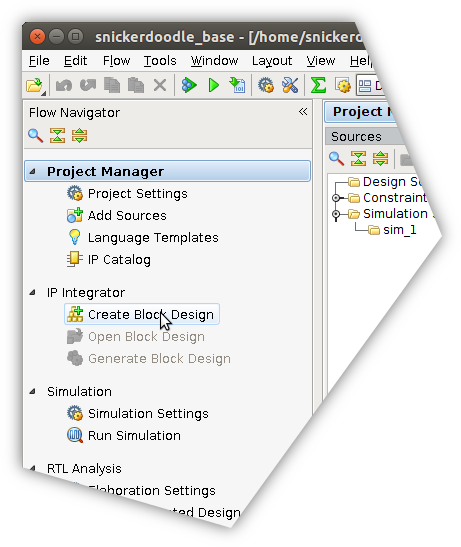
\includegraphics{images/Create_Block_Design.png}
	\caption[Create Block Design]{Create Block Design}
	\label{fig:createblockdesign}
\end{marginfigure}

A block design is a visual representation of the hardware configuration. Hardware configurations can be defined by including or creating sources and assigning hardware I/O. \figref{fig:exampleblockdesign} shows an example block design with hardware definitions for fixed peripherals such as memory interfaces and a soft processing core (MicroBlaze). \\

\begin{figure}
	\centering
	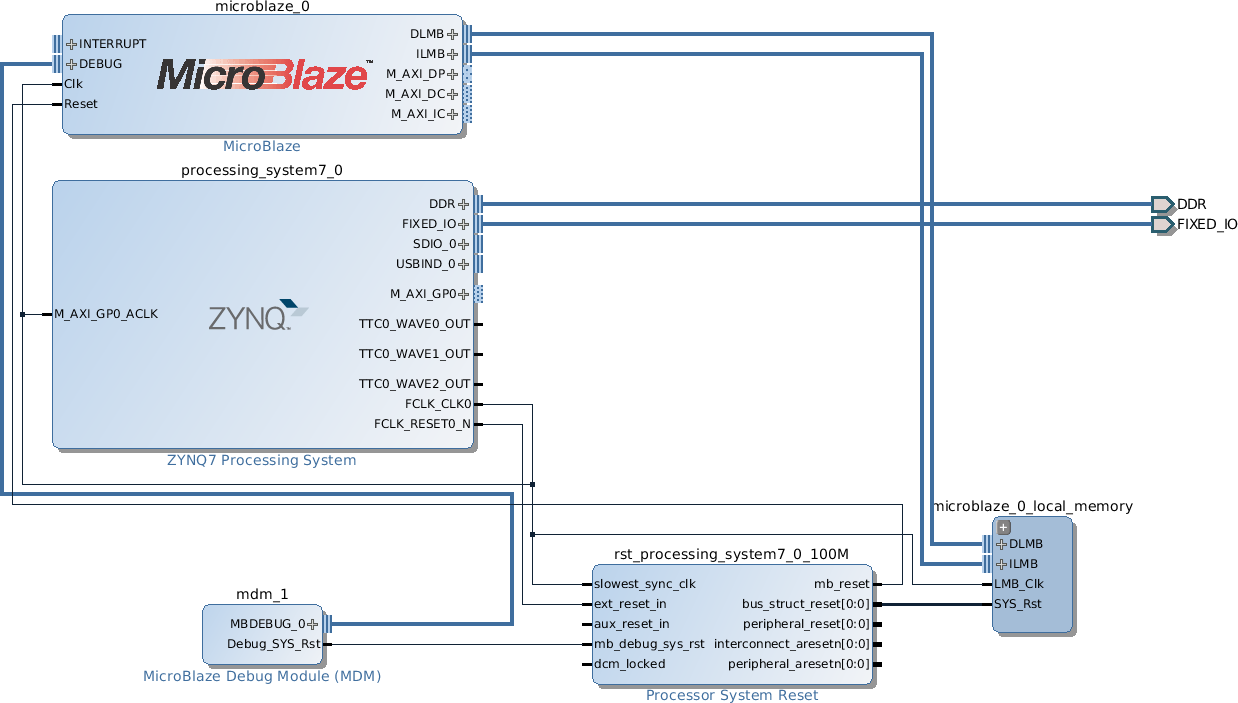
\includegraphics{images/Example_Block_Design.png}
	\caption{Example Block Design with Zynq Processing System and Microblaze Soft Core Processor}
	\label{fig:exampleblockdesign}
\end{figure}

\noindent
To create a block design for a new project, select \textit{\bfseries Flow $\rightarrow$ Create Block Design} from the menubar or from the "IP Integrator" section of the \textit{Flow Navigator} pane as shown in \figref{fig:createblockdesign}. \\

\noindent
Adding and integrating sources and IP into a block design can vary greatly depending on the design and application. For additional reading and information on integrating IP can be found at \url{http://www.xilinx.com/support/documentation/sw_manuals/xilinx2015_4/ug896-vivado-ip.pdf}. 

\newpage

\subsection{Add Sources and IP}
\label{sub:addsources}

Adding sources can be done by right clicking inside the \textit{Sources} pane or by selecting \textit{\bfseries File $\rightarrow$ Add Sources...} from the menubar. The \textit{Add Sources Wizard} will appear and allow you to select existing sources, IP and constraints to add to the project. \\


\begin{figure}
	\centering
	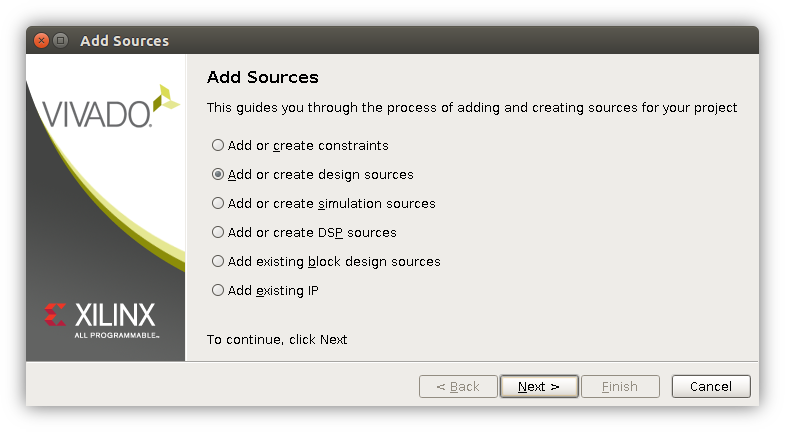
\includegraphics{images/Add_Sources_Dialog.png}
	\caption{Adding New Sources to the Project with the Add Sources Wizard}
	\label{fig:addsourceswiz}
\end{figure}


\subsection{Create HDL Wrapper}

Before generating a bitstream for the project, an HDL wrapper must be generated for the design. To do this, right click on the design (in this case "base\_design") from within the \textit{Sources} pane and select "Create HDL Wrapper...". 


\begin{figure}
	\centering
	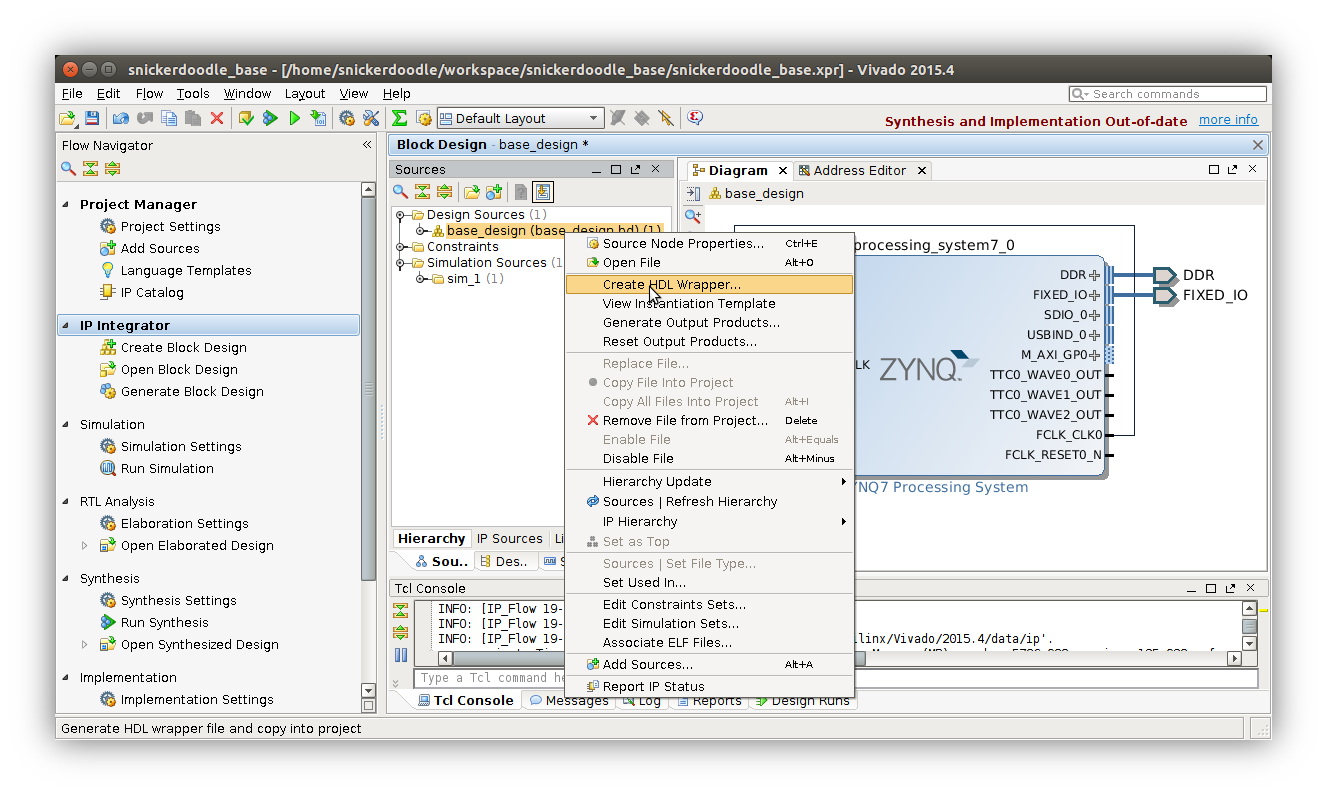
\includegraphics{images/Create_HDL_Wrapper.png}
	\caption{Creating an HDL Wrapper for the Design}
	\label{fig:createhdlwrapper}
\end{figure}


\subsection{Generating Bitstreams}

Bitstreams can be generated by selecting \textit{\bfseries Flow $\rightarrow$ Generate Bitstream} from the menubar or from within the "Program and Debug" section of the \textit{Flow Navigator} pane as shown in \figref{fig:genbitstream}. The bitstream contains all the information necessary to define the programmable logic and the associated hardware peripherals/interfaces.

\begin{marginfigure}
	\centering
	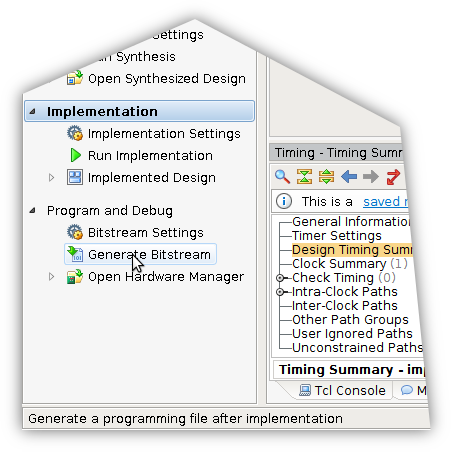
\includegraphics{images/Generate_Bitstream.png}
	\caption[Generate Bitstream from Vivado Flow Navigator]{Generate Bitstream from Vivado Flow Navigator}
	\label{fig:genbitstream}
\end{marginfigure}





\section{Exporting Design with SDK}

\subsection{Export the Hardware Platform}

\begin{marginfigure}
	\centering
	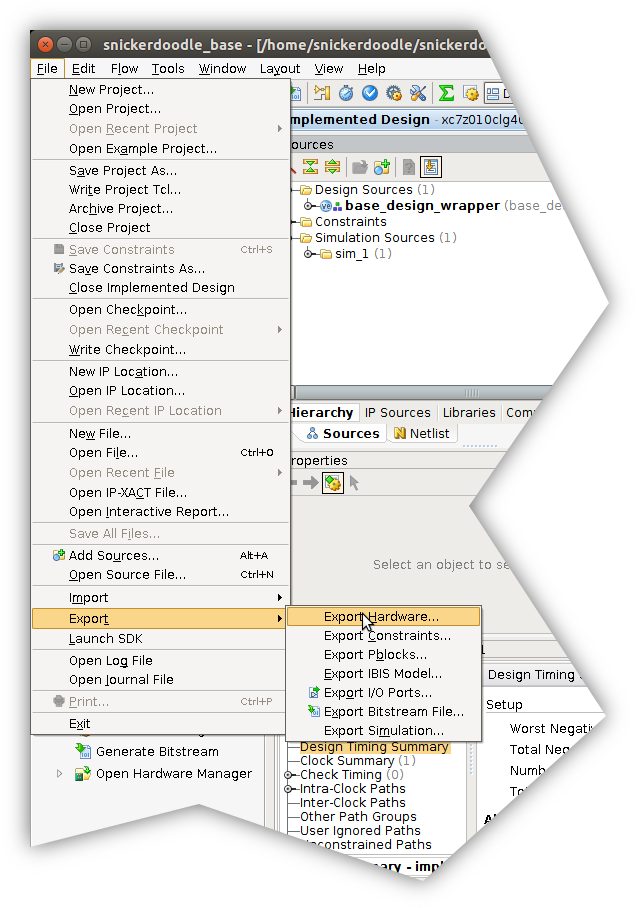
\includegraphics{images/Export_Hardware.png}
	\caption[Export Hardware Configuration from Vivado]{Export Hardware Configuration from Vivado}
	\label{fig:exporthardware}
\end{marginfigure}

Designs that are implemented using Vivado can be exported and opened in the SDK directly from Vivado. Before a design can be opened in the SDK, the hardware profile must be exported which can be done by selecting \textit{\bfseries File $\rightarrow$ Export $\rightarrow$ Export Hardware...} from the menubar as shown in \figref{fig:exporthardware}. \\


\begin{figure}
	\centering
	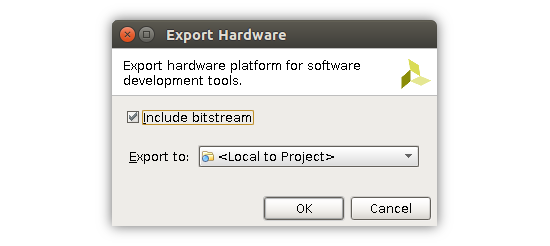
\includegraphics{images/Export_Hardware_Dialog.png}
	\caption{Export Hardware for Software Development Dialog}
	\label{fig:exporthardwaredialog}
\end{figure}

\noindent
\figref{fig:exporthardwaredialog} shows the options for hardware export. Select the "Include bitstream" checkbox to include the bitstream with the hardware definition files for use with the SDK. If you would like to use the hardware platform in a workspace other than the hardware project directory, change the selection of the "Export to:" input. This will be the workspace for the SDK. \\

\infonote{If you choose an export location other than \texttt{<Local to Project>}, the SDK will need to be launched separately from Vivado to access the exported workspace location}


\subsection{Launching the SDK}

The SDK can be launched directly from Vivado to use the exported hardware profile for software development. To launch the SDK from Vivado, select \textit{\bfseries File $\rightarrow$ Launch SDK} from the menubar, as shown in \figref{fig:launchsdk}. If the hardware platform was exported to a directory within the Vivado project (by selecting \texttt{<Local to Project>} as export location), the hardware platform will be immediately available within the SDK workspace. If the hardware was exported to a different directory, you will need to change the workspace directory after the SDK has launched.

\begin{marginfigure}
	\centering
	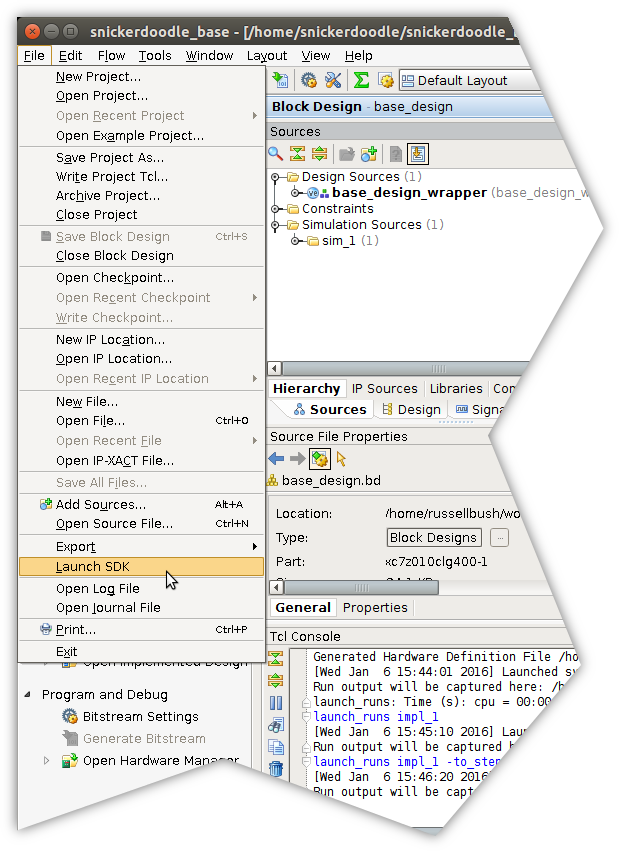
\includegraphics{images/Launch_SDK.png}
	\caption[Launch SDK from Vivado]{Launch SDK from Vivado}
	\label{fig:launchsdk}
\end{marginfigure}


\section{Building Bitstream into \texttt{BOOT.bin}}
Bitstreams can be built into the boot image and specified to be loaded when the boot image starts the boot process. This method can be useful for bitstreams that need to be loaded \textit{before} the operating system is booted. There are two methods for building the boot image (\texttt{BOOT.bin}): a GUI based method executed from the SDK environment and a command line method from which the GUI process is derived. The required components (termed \textit{partitions}), for creating a boot image are as follows:

%\margininfonote{Chapter 3 in the \href{http://www.xilinx.com/support/documentation/user_guides/ug821-zynq-7000-swdev.pdf}{Zynq-7000 All Programmable SoC Software Developers Guide} has more detailed information about the boot process and components of the boot image.}

\begin{description}
	\item[\texttt{fsbl.elf}] - First stage boot loader (FSBL). Responsible for loading the bitstream (if one exists), loading into memory and handing off the boot process to the second stage bootloader.
	\item[\texttt{u-boot.elf}] - Second stage boot loader. Responsible for loading Linux system components (devicetree, uImage, file system)
	\item[\texttt{system.bit}] - The bitstream to be built into the boot image.
	\item[\texttt{devicetree.dtb}] - The Linux devicetree to be loaded by FSBL or U-Boot.
	\item[\texttt{uImage.bin}] - Linux kernel image to be loaded by FSBL or U-Boot.
\end{description}

\subsection{Building Boot Images from SDK}

The SDK provides a graphical way to select the components/partitions for the boot image and generate a \textit{boot image file} (\texttt{.bif}). The graphical front-end provides the necessary interface for selecting existing boot partitions (typically pre-compiled and/or provided by Vivado project) and will generate the \texttt{.bif} file along with the boot image. \figref{fig:createbootimage} shows the graphical interface for creating Zynq boot images from the SDK. To access the interface and begin generating images, select \textit{\bfseries Xilinx Tools $\rightarrow$ Create Boot Image} from the menubar in the SDK. \\

\begin{figure}
	\centering
	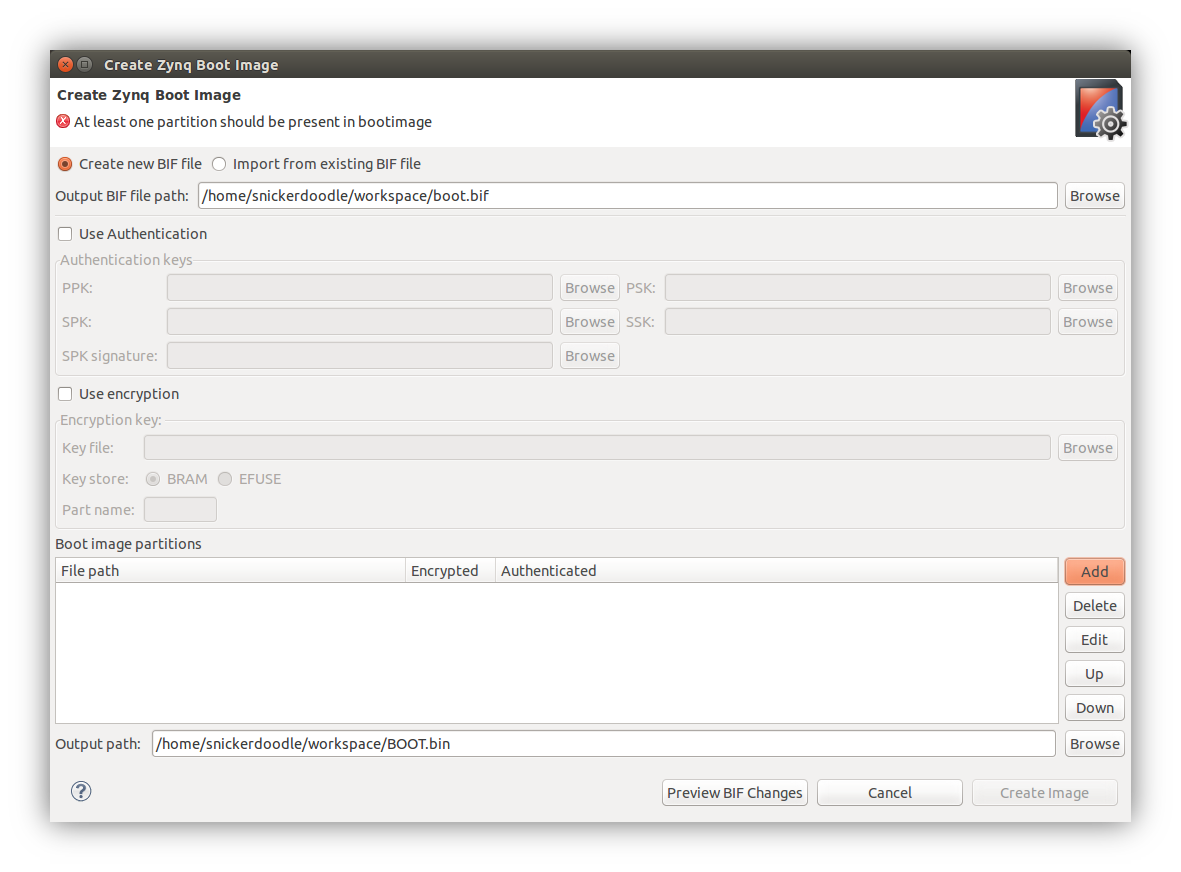
\includegraphics{images/Create_Boot_Image.png}
	\caption{Interface to Create Boot Image from Xilinx SDK}
	\label{fig:createbootimage}
\end{figure}

\noindent
Prebuilt \texttt{.bif} files can be used by the SDK interface by selecting "Import from exisiting BIF file", shown at the top of the window in \figref{fig:createbootimage}. Boot partitions are listed in the "Boot image partitions" table within the interface. To add boot partitions from the interface, selecting "Add" will open an "Add partition" dialog (shown in \figref{fig:bootimagepartition}) which will allow you to select and specify the partition file. \\ 


\begin{marginfigure}
	\centering
	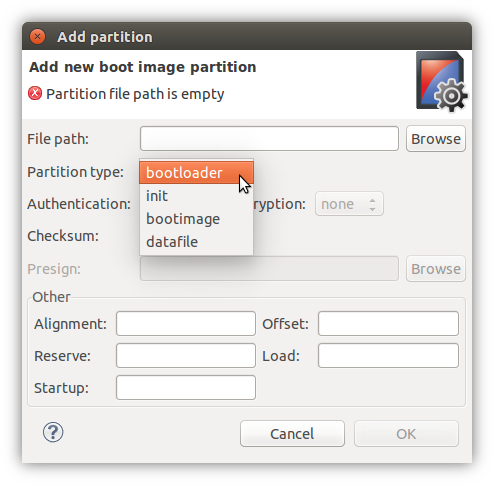
\includegraphics{images/New_Boot_Image_Partition.png}
	\caption[Create New Boot Image Parition]{Create New Boot Image Parition}
	\label{fig:bootimagepartition}
\end{marginfigure}

\newpage

\subsection{Building Boot Images with \texttt{bootgen}}
\margincautionnote{When building boot images with \texttt{bootgen} the boot partition files and \texttt{.bif} file should be isolated in a working directory from which \texttt{bootgen} is executed.}

The GUI interface for building boot images from within the SDK is simply a wrapper for the command line executable that serves the same purpose. \texttt{bootgen} can be provided with a \texttt{.bif} file to specify the boot image partitions. Below is an example \texttt{.bif} file: \\

\begin{lstlisting}[style=text]
image : {
    [bootloader]fsbl.elf
    u-boot.elf
    bitstream.bit
    [load=0x2ff0000]devicetree.dtb
    [load=0x3000000]uImage.bin
}
\end{lstlisting}

~\\
\noindent
After copying the boot partition file and the \texttt{.bif} file to a local working directory, the \texttt{bootgen} utility can be executed from that directory to output the boot image. Invoking the following command will create a boot image named \texttt{BOOT.bin} using the boot image file \texttt{boot.bif}: \\

\begin{lstlisting}[style=text]
bootgen -image boot.bif -o i BOOT.bin
\end{lstlisting}



\section{Loading Bitstream from Linux}
Bitstreams can be loaded to the FPGA from a booted Linux system. This allows bitstreams to be loaded on a system without needing to regenerate a boot image or reboot the system. This can be useful for testing and development.

\subsection{Preparing Bitstream for Loading (bit-reversing)}
The bitstreams must be bit-reversed before  they can be loaded from Linux. The \texttt{-split} argument can be supplied to the \texttt{bootgen} utility to tell it to create a bit-reversed copy of the bitstream that can be loaded from Linux. \\


\begin{lstlisting}
bootgen -image boot.bif -split bin -o i BOOT.bin
\end{lstlisting}

~\\ Using \texttt{-split bin} will append a \texttt{.bin} suffix to the input files specified in the boot image file (\texttt{boot.bif}). In the case of the \texttt{.bif} example above, this will output a new, bit-reversed bitstream named \texttt{bitstream.bit.bin}.


\subsection{Writing Bitstream to Device}
\margincautionnote{Attempting to write bitstreams that have not been reformatted to bit-reversed will not successfully load to \texttt{xdevcfg} and the \texttt{prog\_done} flag will fail to be asserted.}


Now that the bitstream has been bit-reversed, it can be written to the FPGA using the \texttt{xdevcfg} driver. To load the bitstream, write the contents of the bitstream file to the \texttt{xdevcfg} device using the following command: \\

\begin{lstlisting}[style=text]
cat bitstream.bit.bin > /dev/xdevcfg
\end{lstlisting}


~\\
\noindent
Writing the bitstream to the device can take some time. The \texttt{prog\_done} flag can be read to check whether the bitstream has finished loading: \\

\begin{lstlisting}[style=text]
cat /sys/devices/amba.0/f8007000.ps7-dev-cfg/prog_done
1
\end{lstlisting}


~\\
\noindent
This process allows bitstreams to be loaded, and thus the FPGA to be reconfigured, without needing to alter the \textit{BOOT} partition of the SD card (\ie \texttt{BOOT.bin}) or reboot the system. 



